%Version 3.1 December 2024
% See section 11 of the User Manual for version history
%
%%%%%%%%%%%%%%%%%%%%%%%%%%%%%%%%%%%%%%%%%%%%%%%%%%%%%%%%%%%%%%%%%%%%%%
%%                                                                 %%
%% Please do not use \input{...} to include other tex files.       %%
%% Submit your LaTeX manuscript as one .tex document.              %%
%%                                                                 %%
%% All additional figures and files should be attached             %%
%% separately and not embedded in the \TeX\ document itself.       %%
%%                                                                 %%
%%%%%%%%%%%%%%%%%%%%%%%%%%%%%%%%%%%%%%%%%%%%%%%%%%%%%%%%%%%%%%%%%%%%%

%%\documentclass[referee,sn-basic]{sn-jnl}% referee option is meant for double line spacing

%%=======================================================%%
%% to print line numbers in the margin use lineno option %%
%%=======================================================%%

%%\documentclass[lineno,pdflatex,sn-basic]{sn-jnl}% Basic Springer Nature Reference Style/Chemistry Reference Style

%%=========================================================================================%%
%% the documentclass is set to pdflatex as default. You can delete it if not appropriate.  %%
%%=========================================================================================%%

%%\documentclass[sn-basic]{sn-jnl}% Basic Springer Nature Reference Style/Chemistry Reference Style

%%Note: the following reference styles support Namedate and Numbered referencing. By default the style follows the most common style. To switch between the options you can add or remove Numbered in the optional parenthesis. 
%%The option is available for: sn-basic.bst, sn-chicago.bst%  
 
%%\documentclass[pdflatex,sn-nature]{sn-jnl}% Style for submissions to Nature Portfolio journals
%%\documentclass[pdflatex,sn-basic]{sn-jnl}% Basic Springer Nature Reference Style/Chemistry Reference Style
\documentclass[pdflatex,sn-mathphys-num]{sn-jnl}% Math and Physical Sciences Numbered Reference Style
%%\documentclass[pdflatex,sn-mathphys-ay]{sn-jnl}% Math and Physical Sciences Author Year Reference Style
%%\documentclass[pdflatex,sn-aps]{sn-jnl}% American Physical Society (APS) Reference Style
%%\documentclass[pdflatex,sn-vancouver-num]{sn-jnl}% Vancouver Numbered Reference Style
%%\documentclass[pdflatex,sn-vancouver-ay]{sn-jnl}% Vancouver Author Year Reference Style
%%\documentclass[pdflatex,sn-apa]{sn-jnl}% APA Reference Style
%%\documentclass[pdflatex,sn-chicago]{sn-jnl}% Chicago-based Humanities Reference Style

%%%% Standard Packages
%%<additional latex packages if required can be included here>

\usepackage{graphicx}%
\usepackage{multirow}%
\usepackage{amsmath,amssymb,amsfonts}%
\usepackage{amsthm}%
\usepackage{mathrsfs}%
\usepackage[title]{appendix}%
\usepackage{xcolor}%
\usepackage{textcomp}%
\usepackage{manyfoot}%
\usepackage{booktabs}%
\usepackage{algorithm}%
\usepackage{algorithmicx}%
\usepackage{algpseudocode}%
\usepackage{listings}%
%%%%

%%%%%=============================================================================%%%%
%%%%  Remarks: This template is provided to aid authors with the preparation
%%%%  of original research articles intended for submission to journals published 
%%%%  by Springer Nature. The guidance has been prepared in partnership with 
%%%%  production teams to conform to Springer Nature technical requirements. 
%%%%  Editorial and presentation requirements differ among journal portfolios and 
%%%%  research disciplines. You may find sections in this template are irrelevant 
%%%%  to your work and are empowered to omit any such section if allowed by the 
%%%%  journal you intend to submit to. The submission guidelines and policies 
%%%%  of the journal take precedence. A detailed User Manual is available in the 
%%%%  template package for technical guidance.
%%%%%=============================================================================%%%%

%% as per the requirement new theorem styles can be included as shown below
\theoremstyle{thmstyleone}%
\newtheorem{theorem}{Theorem}%  meant for continuous numbers
%%\newtheorem{theorem}{Theorem}[section]% meant for sectionwise numbers
%% optional argument [theorem] produces theorem numbering sequence instead of independent numbers for Proposition
\newtheorem{proposition}[theorem]{Proposition}% 
%%\newtheorem{proposition}{Proposition}% to get separate numbers for theorem and proposition etc.

\theoremstyle{thmstyletwo}%
\newtheorem{example}{Example}%
\newtheorem{remark}{Remark}%

\theoremstyle{thmstylethree}%
\newtheorem{definition}{Definition}%

\raggedbottom
%%\unnumbered% uncomment this for unnumbered level heads

\begin{document}

\title[Cross-setting reliability of AMI anemia prediction]{Cross-setting reliability of anemia prediction after acute myocardial infarction: a retrospective evaluation of observation processes and model transport}


%%==================================%%
%% Sample for unstructured abstract %%
%%==================================%%
\abstract{
\textbf{Background:} Laboratory observation patterns in electronic health records may reflect local care practices as well as patient physiology, potentially limiting the transportability of prediction models. We evaluated whether predictive gains from early laboratory observation features persisted across settings when predicting recorded anemia after acute myocardial infarction (AMI).

\textbf{Methods:} In this retrospective study, models were developed and calibrated using MIMIC-IV 2.2 and evaluated in a diagnosis-triggered cohort from a single hospital in China. Among patients with normal early hemoglobin (Hb), information from calendar days D0--1 was used to predict recorded anemia on D2--7, conditional on future Hb measurement. Public training, calibration, and test sets comprised 1,107, 369, and 370 patients, respectively. Preprocessing, fitted models, and public calibration were frozen before local evaluation. We compared routine-laboratory and observation-augmented models, using an age-, sex-, and Hb-based model as a simple benchmark. Exploratory analyses examined care-pathway composition, observation-feature representation, and outcome ascertainment.

\textbf{Results:} Future Hb measurements were available for 1,846/1,934 eligible public patients and 100/116 eligible local patients, with 839 and 46 recorded-anemia events, respectively. Observation augmentation increased public-test area under the receiver operating characteristic curve (AUROC) from 0.684 to 0.764. In the local cohort, AUROC was 0.728 with augmentation versus 0.785 without (paired difference, $-0.057$; 95\% bootstrap interval, $-0.147$ to 0.017), whereas the Brier score increased by 0.073 (95\% interval, 0.028 to 0.119). The augmented model predicted a mean anemia risk of 64.3\%, compared with an observed event fraction of 46.0\%. The simple benchmark achieved an AUROC of 0.876 but had a calibration slope of 2.79. The public observation-feature advantage was not evident in non-CABG comparisons, while alternative observation encodings altered local probability performance. Explicit modeling of future Hb observation and the joint recorded event did not resolve local risk overestimation.

\textbf{Conclusions:} Internal discrimination gains from laboratory observation features did not establish reliable probability estimates across settings. Care-pathway composition, observation-feature representation, and outcome observability are important considerations when evaluating model transport. Findings are limited by the small, selected single-hospital cohort and exploratory analyses; clinical utility was not established. The study was not registered.
}

\keywords{Acute myocardial infarction, Anemia, Electronic health records, Observation processes, Model transportability, Calibration}
\maketitle

\section{Background}\label{sec1}

Hemoglobin (Hb) decline and hospital-acquired anemia are common during hospitalization for acute myocardial infarction (AMI) and are associated with adverse clinical outcomes \cite{salisbury2010}. Diagnostic blood loss, treatment, and other inpatient processes may contribute to these changes \cite{salisbury2011}, although their frequency and prognostic implications vary across populations and outcome definitions \cite{li2023,colombo2023}. Predicting subsequent laboratory-defined anemia may help characterize inpatient Hb trajectories. However, a recorded threshold crossing does not necessarily indicate clinically significant bleeding or establish anemia status between measurements, and its prediction does not itself demonstrate clinical benefit.

Electronic health records (EHRs) capture both physiological measurements and the processes through which they are obtained. Test availability, timing, and repetition may provide predictive information beyond measured values \cite{agniel2018,sisk2021,che2018}, while also reflecting care pathways, clinical workflows, and recording practices that differ across settings \cite{finlayson2021,wong2021}. Consequently, observation features may improve prediction within a development dataset without preserving their predictive associations elsewhere. Gains in internal discrimination therefore do not necessarily establish the reliability of transported risk estimates.

Laboratory-defined anemia prediction is particularly sensitive to observation processes because measurement affects both predictors and outcome ascertainment. Early testing patterns can inform prediction, whereas subsequent Hb measurements determine whether a recorded anemia event can be evaluated. Patients without future Hb measurements cannot be classified as anemia-free; prediction among remeasured patients therefore concerns a conditional recorded outcome rather than the occurrence of biological anemia in all eligible patients. Previous research has examined inpatient and laboratory prediction tasks \cite{goodwin2020,lindaLi2022,dauvin2019}, while cross-database shifts associated with observation features have also been investigated in sepsis \cite{yamamoto2026}. However, the combined implications of predictor observation, outcome ascertainment, and care-pathway composition for cross-setting probability reliability remain insufficiently characterized in this AMI laboratory task.

We conducted a retrospective cross-setting evaluation of recorded-anemia prediction after AMI using models developed and calibrated in MIMIC-IV 2.2 and applied without refitting to a selected single-hospital cohort in China. The primary objective was to assess whether adding early laboratory observation features to routine physiological measurements provided a transferable predictive advantage, using an age-, sex-, and Hb-based model as a benchmark. We evaluated discrimination, probability error, and calibration, with exploratory analyses addressing care-pathway composition, observation-feature representation, and future outcome observation. This approach examined the reliability of transported EHR predictions rather than the development of a new prediction algorithm.

\section{Methods}

\subsection{Study design, data sources, and cohort selection}

We conducted a retrospective cross-setting evaluation of electronic health record (EHR)-based models for recorded anemia after acute myocardial infarction (AMI). Models were developed and calibrated in MIMIC-IV version 2.2 and externally evaluated, without refitting, in a single-hospital cohort from China. The evaluation included frozen-model performance assessment, exploratory analyses of care pathways and laboratory observation patterns, and supporting sensitivity analyses (Fig.~\ref{fig:design}).

MIMIC-IV version 2.2 provided the public data from the United States (2008--2019) \cite{mimicpaper,mimicdata}. Local data were obtained from Anhui Chest Hospital, Hefei, China, through an EHR export triggered by a primary or secondary discharge diagnosis of AMI, including ST-elevation and non-ST-elevation AMI. The export imposed no additional procedure, transfusion, or departmental restrictions and could include other admissions of selected patients. It comprised 399 patients and 436 admissions, with available admission dates from 18 October 2019 to 2 December 2025 and discharges through 15 January 2026. Complete capture of all hospital AMI admissions during this period was not established.

For each adult patient, the first visible admission with a primary diagnosis of acute coronary syndrome (ACS) was identified before applying hemoglobin (Hb) eligibility criteria. A linked historical coronary export was used to identify earlier visible ACS admissions without imposing its treatment-based selection criteria on the main cohort. The analysis was restricted to index admissions with a primary AMI diagnosis. Public AMI was identified using primary ICD-9 prefix 410 or ICD-10 prefixes I21 and I22; local AMI and ACS were identified from discharge-diagnosis text, excluding suspected diagnoses and conflicting primary diagnoses. No additional study-specific clinical adjudication was performed.

After cohort selection, 116 local patients met the early-normal Hb eligibility criteria, of whom 100 had future Hb measurements and contributed to the primary conditional-anemia evaluation. The remaining 16 had unknown conditional outcomes. The detailed selection process is reported in Table~S1 and Fig.~S6 (Additional file 1).

The local cohort was evaluated as a single retrospective sample without local development or validation subsets. Primary models and public calibration procedures were frozen before local evaluation. Care-pathway and observation-representation analyses were exploratory and post-hoc, informed by local findings, and did not involve refitting the primary models. Reporting was guided by TRIPOD+AI and RECORD recommendations \cite{tripodai,record2015}.

\begin{figure*}[!t]
\centering
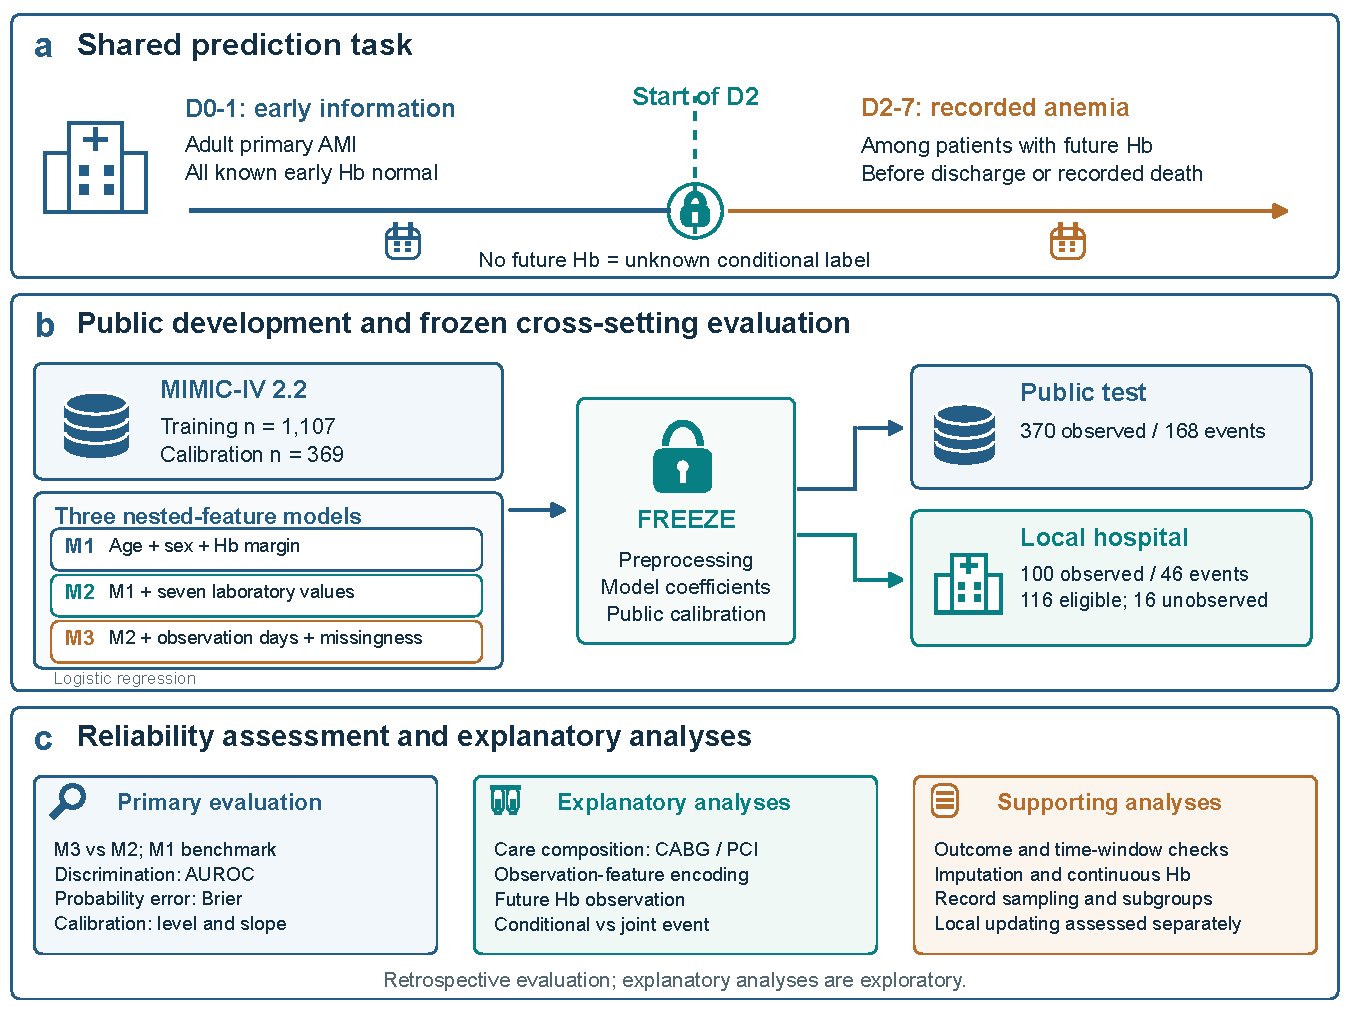
\includegraphics[width=\textwidth]{figures/Figure1_reliability_vector.pdf}
\caption{Framework for early recorded-anemia prediction and frozen cross-setting evaluation. Panels a--c illustrate the prediction timeline, model development and evaluation, and analysis hierarchy.}
\label{fig:design}
\end{figure*}

\subsection{Prediction landmark and outcome definitions}

Admission was designated calendar day D0, and prediction occurred at the beginning of D2 using information from D0--1, rather than after exactly 48 elapsed hours. Eligibility required adult age, known sex, an interpretable admission--discharge sequence, hospitalization beyond the D2 date boundary, and at least one valid early Hb measurement. All interpretable D0--1 Hb values were required to be at least 130~g/L in men or 120~g/L in women, using fixed adult anemia thresholds \cite{who2024}. Patients with uninterpretable early Hb values were excluded, and age was capped at 90 years. Local admissions discharged on D2 were excluded because exact discharge times were unavailable.

Among eligible patients, future Hb observation was defined as $O=1$ when at least one valid Hb result was recorded during D2--7 before discharge or recorded death. Public outcomes used specimen timestamps, whereas local outcomes used laboratory report dates. Recorded anemia ($A$) was evaluated only when $O=1$: $A=1$ indicated any future Hb measurement below the sex-specific threshold, and $A=0$ indicated no threshold crossing among available measurements. Patients with $O=0$ were not assigned negative conditional-anemia labels.

For early predictors $X$, the primary prediction target was

\begin{equation}
q(X)=\Pr(A=1\mid O=1,X).
\end{equation}

We additionally defined the joint recorded endpoint $J=1$ when both future Hb observation and recorded anemia occurred, and $J=0$ otherwise. Its probability was expressed as

\begin{equation}
\begin{aligned}
r(X)&=\Pr(J=1\mid X)=o(X)q(X),\\
o(X)&=\Pr(O=1\mid X).
\end{aligned}
\end{equation}

Thus, $J=0$ in patients without future Hb indicates no recorded event, not biological normality. Neither endpoint identifies anemia between measurements or determines anemia status among patients without future Hb. Additional outcome-implementation details are provided in Supplementary Methods S1.

\subsection{Laboratory harmonization, predictors, and model development}

Eight laboratory variables were used: Hb, creatinine, albumin, white blood cell count, platelet count, sodium, potassium, and glucose. Measurements were standardized to g/L for Hb and albumin, $\mu$mol/L for creatinine, $10^9$/L for white blood cells and platelets, and mmol/L for sodium, potassium, and glucose. Local units were confirmed by the researcher and supported by overlapping unit-bearing historical records. Public measurements were converted accordingly. Specimen restrictions, plausibility bounds, deduplication, and handling of missing or uninterpretable values are detailed in Supplementary Methods S1 and Table~S2.

Public early predictors required D0--1 specimen collection and result availability before D2, using the later of \texttt{charttime} and \texttt{storetime}. Local records had calendar-date precision only, precluding equivalent within-day availability checks. The latest early daily median supplied each laboratory value, while all valid early Hb measurements were considered for eligibility. Observation-day counts represented distinct calendar days with available measurements (0--2), rather than the number of blood draws.

Public outcome-observed AMI patients were divided into training ($n=1,107$), calibration ($n=369$), and held-out test ($n=370$) sets. Five models were evaluated. M0 used the latest early Hb margin above the sex-specific threshold; M1 added age and sex; and M2 added seven routine laboratory values. M3 extended M2 with eight observation-day counts and ten missingness indicators. M4 used histogram gradient boosting with the M2 physiological inputs.

M0--M3 used logistic regression ($C=1$), with median imputation and standardization fitted exclusively on public training data. M4 used 150 boosting iterations and a learning rate of 0.05; leaf number and L2 regularization were selected by three-fold public-training cross-validation. Model log-odds were subsequently calibrated using logistic regression in the separate public calibration set. All preprocessing parameters, fitted models, and calibration transformations remained unchanged during public testing and local evaluation. No local outcomes were used to select, recalibrate, or refit the primary models. Models were implemented in scikit-learn \cite{sklearn2011}. Further specifications are provided in Supplementary Methods S2; complete feature and model dictionaries are available in the accompanying repository.

\subsection{Care-pathway composition and observation-representation analyses}

Exploratory analyses examined the sensitivity of observation-feature performance to care-pathway composition and feature representation.

Public coronary artery bypass grafting (CABG) and percutaneous coronary intervention (PCI) groups were defined using admission-wide procedure codes, with CABG taking precedence. These retrospective classifications were not used as early predictors. M2 and M3 were compared in the full public test set and among the same 290 non-CABG test patients, first using the frozen full-cohort models and then using previously fitted public non-CABG redevelopment models. Restriction altered evaluation composition, whereas redevelopment also altered training composition; neither comparison identified causal mediation.

Local care-pathway analyses used procedure-name evidence linked by patient and admission, with operative notes prioritized when available. Incomplete note coverage and date-only procedure records limited treatment ascertainment. Absence of a recorded procedure was not interpreted as verified treatment absence. Transfusion evidence was derived from relevant procedure entries and notes; missing timing and volume information prevented reliable dose-related analyses. Procedures and transfusions were used only for retrospective characterization and sensitivity analyses, not as predictors. Source-specific ascertainment limitations are described in Supplementary Methods S1, with local pathway summaries in Table~S7.

Alternative observation representations were evaluated using public-fitted, publicly calibrated models. A4 retained albumin concentration but removed its observation-day count and missingness input. B2 combined M2 physiological variables with indicators of laboratory measurement on at least two early days, without separate missingness flags. Other ablation and representation variants are defined in Supplementary Methods S2, with performance estimates and paired comparisons in Tables~S4--S5. These post-hoc comparisons were informed by local findings and did not constitute independent validation of replacement models.

\subsection{Outcome observation and supporting analyses}

Separate public-fitted observation models O1--O3 used the feature sets corresponding to M1--M3 to predict future Hb observation. The 88 public patients without future Hb were allocated to training, calibration, and test subsets (52, 18, and 18, respectively), yielding observation-model sample sizes of 1,159, 387, and 388. Joint recorded-event probabilities J1--J3 were calculated by multiplying the corresponding frozen observation and conditional-anemia probabilities, without local or joint-endpoint recalibration. These models addressed recorded-event ascertainment rather than unmeasured biological anemia (Table~S6).

Supporting analyses varied the recorded outcome definition, follow-up window, and eligibility criteria. Alternative outcomes included future daily-median or last-day Hb, Hb below 110~g/L, and Hb decline of at least 20~g/L. Additional analyses required an early Hb margin of at least 10~g/L or restricted observation to D2--3 or D2--5. Patients without Hb measurements within shortened windows retained unknown conditional labels. A separate D3 landmark analysis used a previously developed public D3 model. Other sensitivities examined iterative imputation, public-period and non-CABG development, recent local admissions, sex, early repeat testing, and exclusions based on recorded CABG or transfusion evidence. These analyses are detailed in Supplementary Methods S2 and Tables~S8--S9.

Previously fitted public Ridge regression models ($\alpha=1$) were evaluated for continuous recorded Hb nadir, signed decline, and nadir margin, using a public-training-median constant as a comparator and retaining public-calibration mean-residual correction (Table~S10). Observation-weighted analyses applied inverse probabilities from the frozen public O3 model, clipped below at 0.05 or 0.10; their missingness and transport assumptions were not established (Table~S11). In 200 record-sampling simulations, one future Hb result per patient and calendar day was retained to assess sensitivity to available measurements (Table~S12).

Exploratory local updating was evaluated separately from frozen transport using ten repetitions of five-fold cross-fitting, with intercept-only or intercept-and-slope adjustment (Table~S14). Five-fold dataset-origin classifiers assessed public--local feature separability rather than anemia prediction (Table~S15). Public development-bootstrap and repeated-split analyses assessed development-sample variation but did not quantify full development uncertainty in local evaluation (Tables~S16--S17).

\subsection{Statistical analysis and reproducibility}

Performance measures included the area under the receiver operating characteristic curve (AUROC), average precision, Brier score, mean predicted probability, and calibration intercept and slope \cite{steyerberg2010,steyerberg2014,saito2015}. AUROC measured discrimination, whereas Brier score assessed overall probability error. Mean predicted risk was compared with the observed event fraction to assess average alignment, independently of calibration across the risk distribution.

The primary comparison was M3 versus M2, isolating the additional contribution of observation features; M1 served as a simple clinical benchmark. Performance intervals and paired differences were estimated from 1,000 patient-level bootstrap resamples, using identical patient draws across models within each population. Percentile intervals conditioned on the frozen public-fitted models and did not incorporate complete development uncertainty.

Calibration diagnostics used 1,000 patient-level bootstrap resamples. Calibration plots summarized event fractions within five model-specific prediction quantiles, with pointwise Wilson intervals. Further calibration diagnostics are reported in Table~S13. All comparisons were exploratory without multiplicity adjustment; the analysis hierarchy did not imply prospective specification.

No prospective sample-size or precision calculation was performed, and the limited local sample constrained performance estimation \cite{rileysize,rileyvalidation}. Computational checks assessed patient linkage, allocation integrity, temporal predictor availability, and frozen-prediction consistency. The repository package contains analysis code, feature and model dictionaries, aggregate results, and figure-source data; individual-level hospital records, patient identifiers, predictions, and fitted binary model objects are excluded. Repository accessibility and data-use restrictions are addressed separately in the Availability of data and materials statement.

\section{Results}

\subsection{Cohort characteristics and observation-dependent outcomes}

Among 1,934 early-normal eligible patients with AMI in the public cohort, 1,846 (95.4\%) had future Hb measurements, of whom 839 (45.4\%) had recorded anemia. The joint recorded-event fraction was 43.4\% (839/1,934). In the held-out public test sample, future Hb was observed in 370 of 388 eligible patients, with 168 recorded-anemia events.

Of 436 admissions from 399 patients in the local export, 320 had a primary AMI diagnosis. Index-admission selection, linked visible-history assessment, and application of the D2 discharge-date boundary yielded 280 primary-AMI index patients, of whom 116 met early-normal Hb eligibility criteria. Future Hb was available for 100 patients (86.2\%), including 46 recorded-anemia events (46.0\%); the joint event fraction was 39.7\% (46/116). The remaining 16 patients had unknown conditional-anemia outcomes. Cohort characteristics are presented in Table~\ref{tab:characteristics}, with the detailed selection process in Table~S1 and Fig.~S6 (Additional file 1).

\begin{table*}[!t]
\caption{Cohort characteristics and outcome ascertainment}
\label{tab:characteristics}
\centering
\footnotesize
\setlength{\tabcolsep}{3pt}
\begin{tabular}{p{4.5cm}ccc}
\toprule
& Public AMI & Public test & Local AMI\\
\midrule
Early-normal eligible, n
& 1934 & 388 & 116\\
Future Hb observed, n (\%)
& 1846/1934 (95.4) & 370/388 (95.4) & 100/116 (86.2)\\
Conditional anemia, events/observed (\%)
& 839/1846 (45.4) & 168/370 (45.4) & 46/100 (46.0)\\
Joint recorded event, events/eligible (\%)
& 839/1934 (43.4) & 168/388 (43.3) & 46/116 (39.7)\\
Age, years
& 66.0 (56.0--74.0) & 64.0 (54.2--72.8) & 63.5 (54.0--73.2)\\
Male, n (\%)
& 1294 (70.1) & 257 (69.5) & 82 (82.0)\\
Early Hb, g/L
& 139.0 (132.0--147.0) & 139.0 (132.0--146.8) & 139.0 (133.0--147.0)\\
Albumin measured, n (\%)
& 454/1846 (24.6) & 95/370 (25.7) & 97/100 (97.0)\\
Two early Hb days, n (\%)
& 559/1846 (30.3) & 122/370 (33.0) & 15/100 (15.0)\\
\bottomrule
\end{tabular}

\vspace{2mm}
\parbox{\textwidth}{\footnotesize
\textit{Note:} Continuous characteristics are median
(interquartile range) among outcome-observed patients.
The public test sample is a subset of the overall public cohort.
Patients without future Hb measurements were not assigned
conditional-anemia labels.
}
\end{table*}

The public and local cohorts had similar median early Hb concentrations but differed in laboratory observation patterns. Albumin availability was substantially higher locally, whereas Hb measurement on both early calendar days was less frequent (Table~\ref{tab:characteristics}). Detailed laboratory characteristics and observation frequencies are provided in Table~S3.

\subsection{Frozen model performance across settings}

In public testing, observation augmentation increased AUROC from 0.684 (95\% bootstrap interval, 0.630--0.736) for M2 to 0.764 (0.715--0.813) for M3, with a paired difference of 0.080 (0.038 to 0.120). The corresponding Brier score decreased from 0.222 to 0.199. M4 achieved a similar AUROC of 0.760.

In the local cohort, M3 had an AUROC of 0.728, compared with 0.785 for M2 and 0.876 for the simpler M1 benchmark (Table~\ref{tab:frozen}; Fig.~\ref{fig:performance}). The paired M3-minus-M2 AUROC difference was $-0.057$ ($-0.147$ to 0.017), whereas the M3-minus-M1 difference was $-0.148$ ($-0.250$ to $-0.059$). Thus, the public observation-feature advantage did not translate into demonstrable incremental local discrimination over M2.

\begin{table*}[!t]
\caption{Performance of frozen conditional-anemia models}
\label{tab:frozen}
\centering
\footnotesize
\setlength{\tabcolsep}{3pt}
\begin{tabular}{lcccc}
\toprule
Model & AUROC (95\% interval) & Brier (95\% interval)
& Mean risk (\%) & Slope\\
\midrule
\multicolumn{5}{l}{\textit{Public test: 370 patients / 168 events}}\\
M0 & 0.612 (0.552--0.670) & 0.246 (0.229--0.263) & 45.9 & 0.47\\
M1 & 0.657 (0.603--0.710) & 0.230 (0.215--0.246) & 43.9 & 0.81\\
M2 & 0.684 (0.630--0.736) & 0.222 (0.207--0.239) & 43.9 & 0.91\\
M3 & 0.764 (0.715--0.813) & 0.199 (0.181--0.216) & 44.1 & 1.10\\
M4 & 0.760 (0.709--0.811) & 0.197 (0.179--0.215) & 43.6 & 1.14\\
\midrule
\multicolumn{5}{l}{\textit{Local AMI: 100 patients / 46 events}}\\
M0 & 0.841 (0.765--0.909) & 0.179 (0.156--0.202) & 47.7 & 2.38\\
M1 & 0.876 (0.800--0.939) & 0.173 (0.153--0.197) & 45.9 & 2.79\\
M2 & 0.785 (0.685--0.872) & 0.195 (0.169--0.224) & 45.3 & 1.52\\
M3 & 0.728 (0.617--0.832) & 0.269 (0.223--0.315) & 64.3 & 0.54\\
M4 & 0.736 (0.628--0.832) & 0.246 (0.212--0.281) & 62.9 & 1.39\\
\bottomrule
\end{tabular}

\vspace{2mm}
\parbox{\textwidth}{\footnotesize
\textit{Note:} M0, Hb-margin model; M1, age-, sex-, and Hb-based
model; M2, routine-laboratory model; M3, observation-augmented
model; M4, histogram gradient-boosting model. Models and
calibrators were frozen before local evaluation.
Intervals condition on the fitted public models.
}
\end{table*}

The local probability-error difference was more pronounced. M3 predicted a mean risk of 64.3\% against an observed event fraction of 46.0\%, with a Brier score of 0.269 versus 0.195 for M2. The paired Brier difference was 0.073 (0.028 to 0.119). M1 achieved the lowest local Brier score (0.173), with mean predicted risk of 45.9\%. However, its calibration slope was 2.79 (1.77--4.78), compared with 0.54 (0.07--1.72) for M3, indicating that average risk alignment alone did not establish calibration across the prediction range. The evidence therefore supported greater local probability error with M3 than M2, while the corresponding discrimination difference remained uncertain. Complete paired comparisons and calibration intervals are reported in Tables~S5 and S13.

\begin{figure*}[!t]
\centering
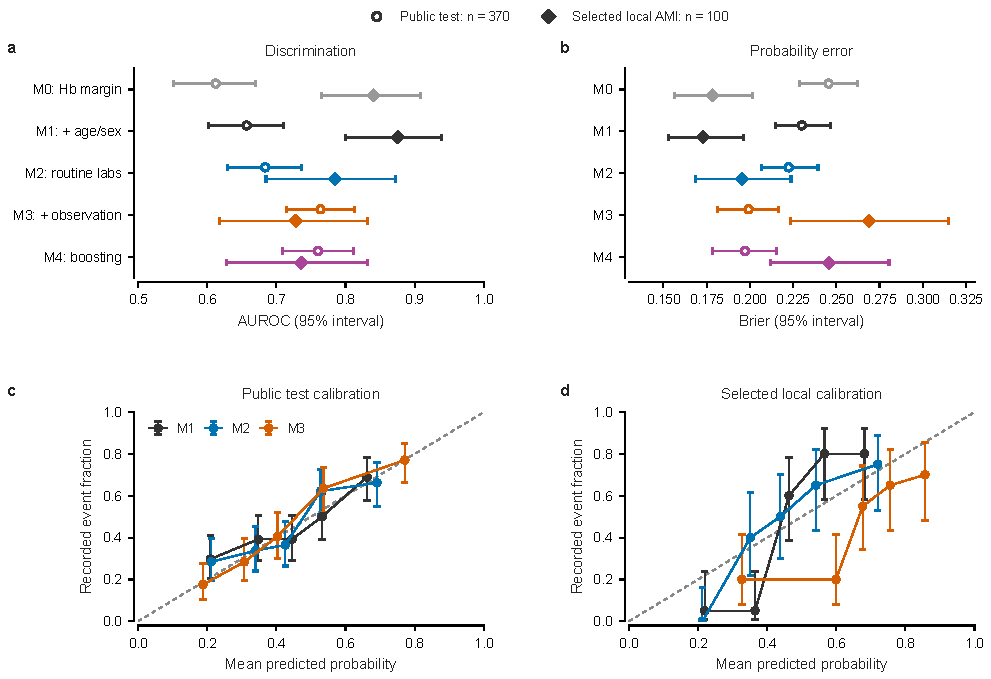
\includegraphics[width=\textwidth]{figures/Figure2_frozen_performance.pdf}
\caption{Frozen-model discrimination, probability error, and calibration in public testing and local AMI evaluation. Panels a--d show AUROC, Brier score, and calibration summaries across settings.}
\label{fig:performance}
\end{figure*}

\subsection{Care-pathway composition and observation-feature gains}

Recorded-anemia frequency differed markedly across public procedure-code groups. Among 1,846 outcome-observed patients, anemia was recorded in 367/379 patients with CABG (96.8\%), 317/1,024 with PCI but no CABG (31.0\%), and 155/443 with neither code (35.0\%). CABG accounted for 21.6\% (80/370) of public test patients but 46.4\% (78/168) of recorded-anemia events (Fig.~\ref{fig:pathway}).

The public observation-feature increment was not apparent after restriction to non-CABG patients. Among the same 290 non-CABG test patients (90 events), frozen M2 and M3 AUROCs were 0.770 and 0.761, respectively, with a paired difference of $-0.009$ ($-0.051$ to 0.031). Corresponding non-CABG redevelopment models achieved AUROCs of 0.808 and 0.803, with a paired difference of $-0.005$ ($-0.022$ to 0.012). These comparisons demonstrated sensitivity to evaluation and development composition without identifying a causal contribution of CABG.

\begin{figure*}[!t]
\centering
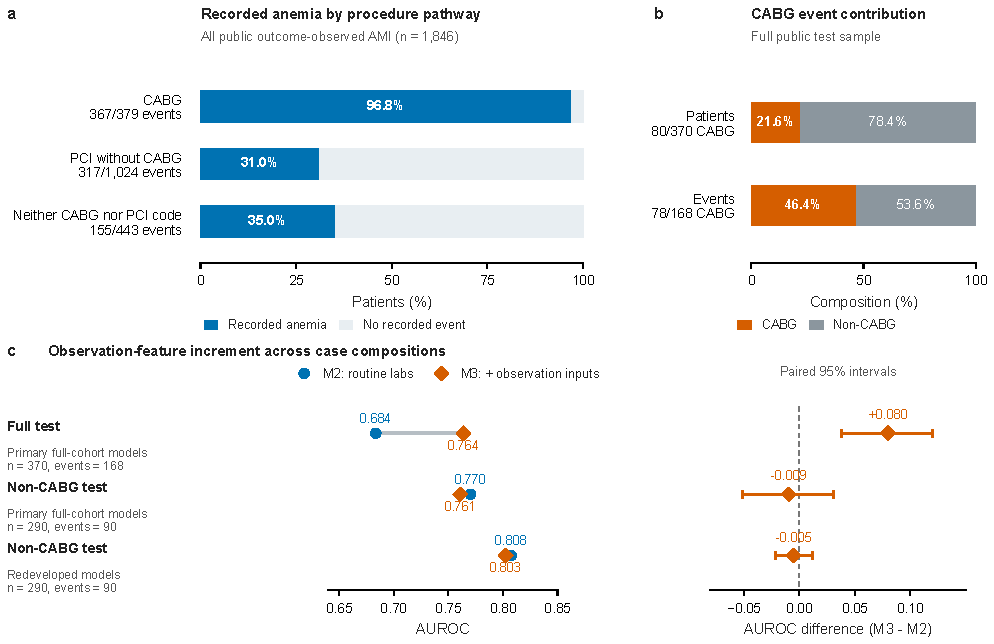
\includegraphics[width=\textwidth]{figures/Figure3_pathway_dependence.pdf}
\caption{Public care-pathway composition and observation-feature discrimination. Panels a--c show procedure-associated event fractions, CABG contributions to test-set composition, and full-cohort versus non-CABG model comparisons.}
\label{fig:pathway}
\end{figure*}

Locally, 82/100 patients had PCI-name evidence and one had CABG-name evidence. Excluding patients with recorded CABG or transfusion evidence did not materially alter the main local performance pattern (Tables~S7--S8). Incomplete treatment ascertainment prevented interpretation of the remaining patients as verified surgery-free or untreated controls.

\subsection{Observation-feature representation and probability behavior}

Early albumin was available in 454/1,846 public outcome-observed patients (24.6\%) versus 97/100 locally (97.0\%) (Fig.~\ref{fig:ablation}). In public testing, M3 mean predicted risk was 44.1\%, close to the observed event fraction of 45.4\%; locally, M3 overestimated the event fraction by 18.3 percentage points. Post-hoc comparisons examined whether alternative observation representations changed this pattern.

A4, which retained albumin concentration but removed its observation inputs, reduced local mean predicted risk from 64.3\% to 44.7\% and Brier score from 0.269 to 0.233. However, AUROC decreased from 0.728 to 0.696 locally and from 0.764 to 0.709 in public testing. The paired local Brier difference relative to M3 was $-0.036$ ($-0.075$ to 0.001), leaving its probability-error advantage uncertain.

The B2 representation yielded local AUROC 0.766, Brier score 0.202, and mean predicted risk 47.7\%. Its paired Brier difference relative to M3 was $-0.066$ ($-0.112$ to $-0.021$). These findings showed that observation-feature representation influenced cross-setting probability performance, but neither post-hoc alternative was independently validated as a replacement model. Results for all evaluated representations, including unfavorable comparisons, are provided in Tables~S4--S5.

\begin{figure*}[!t]
\centering
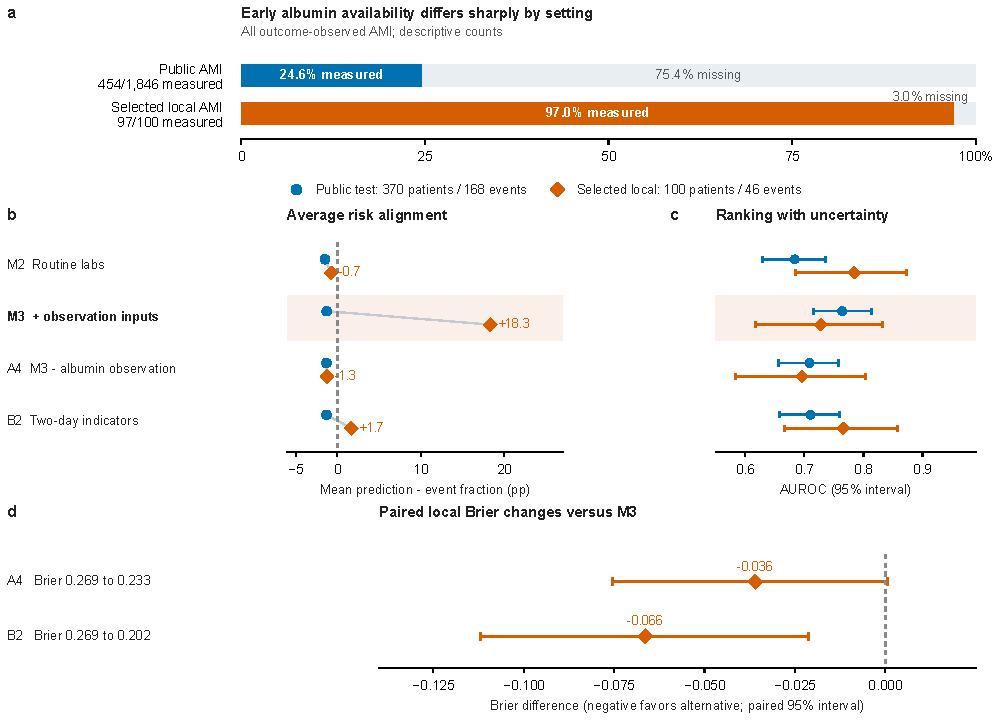
\includegraphics[width=\textwidth]{figures/Figure4_albumin_representation.pdf}
\caption{Laboratory observation patterns and performance under alternative feature representations. Panels a--d show albumin availability, mean-risk alignment, AUROC, and paired local Brier differences relative to M3.}
\label{fig:ablation}
\end{figure*}

\subsection{Future observation, joint recorded events, and supporting analyses}

Future Hb observation was less frequent locally than in the public cohort (86.2\% versus 95.4\%). The public-fitted O3 model achieved a local AUROC of 0.632 (0.465--0.792) and predicted mean observation probability of 95.9\%, exceeding the observed fraction by 9.7 percentage points (Table~\ref{tab:twostage}). Observation-model performance was imprecisely estimated because only 16 local patients lacked future Hb measurements.

For the joint recorded endpoint, J3 predicted mean local risk of 61.2\%, compared with an observed event fraction of 39.7\% and a mean prediction of 43.6\% for J1. Local Brier scores were 0.273 for J3 and 0.182 for J1. Joint-event modeling therefore distinguished the observable target from conditional anemia without resolving overestimation by the observation-augmented model. Complete observation and joint-event results are reported in Table~S6 and illustrated in Fig.~S5.

\begin{table*}[!t]
\caption{Performance of future-observation and joint recorded-event models}
\label{tab:twostage}
\centering
\footnotesize
\setlength{\tabcolsep}{3pt}
\begin{tabular}{lccc}
\toprule
Model & AUROC (95\% interval) & Brier & Mean risk (\%)\\
\midrule
\multicolumn{4}{l}{\textit{Future observation (O): Public eligible test, 388 patients / 370 observed}}\\
O1 & 0.560 (0.418--0.708) & 0.044 & 95.3\\
O3 & 0.636 (0.523--0.739) & 0.044 & 95.3\\
\multicolumn{4}{l}{\textit{Future observation (O): Local AMI, 116 patients / 100 observed}}\\
O1 & 0.521 (0.353--0.704) & 0.127 & 95.3\\
O3 & 0.632 (0.465--0.792) & 0.128 & 95.9\\
\multicolumn{4}{l}{\textit{Joint recorded event (J): Public eligible test, 388 patients / 168 events}}\\
J1 & 0.661 (0.603--0.718) & 0.227 & 41.6\\
J3 & 0.764 (0.716--0.810) & 0.198 & 41.7\\
\multicolumn{4}{l}{\textit{Joint recorded event (J): Local AMI, 116 patients / 46 events}}\\
J1 & 0.826 (0.747--0.898) & 0.182 & 43.6\\
J3 & 0.718 (0.616--0.809) & 0.273 & 61.2\\
\bottomrule
\end{tabular}

\vspace{2mm}
\parbox{\textwidth}{\footnotesize
\textit{Note:} O models predict future Hb observation; J models
combine frozen observation and conditional-anemia probabilities.
Both endpoints use all eligible patients. Absence of a recorded
event does not establish biological normality.
}
\end{table*}

For the 16 local patients without future Hb, assigning all unknown conditional labels as negative or positive would yield event fractions of 39.7\% (46/116) and 53.4\% (62/116), respectively. These are hypothetical missing-label completion limits, not bounds on biological anemia incidence or uncertainty intervals for the observed joint endpoint.

Supporting analyses broadly preserved the unfavorable local probability performance of observation-augmented models. Alternative public development specifications, including iterative imputation and public-period models, showed similar patterns (Table~S9). The separate D3 analysis included 82 patients with 36 recorded-anemia events and was not directly comparable with the D2 cohort.

Continuous-outcome evaluation also showed poorer local performance with observation-rich predictors. For future recorded Hb nadir, mean absolute error was 9.09~g/L for the clinical Ridge model (R1) versus 20.68~g/L for the observation-augmented model (R3); Hb-decline prediction remained limited (Table~S10). Additional endpoint, subgroup, weighting, record-sampling, local-updating, and dataset-origin analyses are detailed in Tables~S8, S11--S12, and S14--S17. None changed the primary frozen-model evaluation.

\section{Discussion}

\subsection{Principal findings}

Laboratory observation features improved discrimination in public testing but did not provide reliable probability estimates in the selected local AMI cohort. Compared with the routine-laboratory model, observation augmentation increased local Brier error and overestimated the recorded-anemia event fraction by 18.3 percentage points. The paired AUROC difference included zero, providing stronger evidence for deterioration in probability accuracy than for a definite reduction in discrimination. The simpler age-, sex-, and Hb-based model achieved better local discrimination and closer average risk alignment, although its calibration slope remained substantially above one.

Exploratory analyses suggested that model behavior was sensitive to care-pathway composition and observation-feature representation. The public discrimination advantage was not evident in non-CABG comparisons, while alternative encodings changed local probability performance. Differences in albumin availability and future Hb observation further highlighted that both predictor measurement and outcome ascertainment may vary across settings. These findings characterize potential sources of transport instability without establishing their causal contributions.

\subsection{Observation processes and care pathways}

Informative observation is well recognized in EHR-based prediction \cite{sisk2021,agniel2018,yamamoto2026}. This study extends its evaluation to a laboratory task in which observation patterns influence both model inputs and the availability of recorded outcomes. Such patterns may reflect patient physiology alongside clinical decisions and data-recording practices. Their failure to transport therefore does not necessarily imply that the original associations were spurious.

The CABG comparisons indicated sensitivity to case composition, but admission-wide procedure codes were not available as early predictors, and subgroup comparisons could not identify causal mediation. Similarly, differences in albumin availability may reflect testing practices or data capture rather than physiological differences alone. Removing albumin observation inputs improved average local risk alignment but reduced AUROC in both settings, with uncertain Brier improvement. The coarser B2 representation showed more favorable local probability performance. These post-hoc findings suggest that feature representation matters, without identifying a causal effect of testing or establishing a validated alternative model.

\subsection{Implications for prediction-model evaluation}

Transported EHR prediction models should be assessed beyond discrimination alone. Simple clinical benchmarks, probability error, calibration, and outcome observability provide complementary evidence about whether predicted risks remain meaningful in a new setting. Neither high AUROC nor agreement between mean predicted risk and event frequency guarantees calibration across the risk distribution \cite{vancalster2019,vancalster2016}. The local M1 results illustrate this distinction, with strong discrimination and close average risk alignment despite a calibration slope substantially above one.

The findings also emphasize the importance of specifying what a model predicts. Conditional recorded anemia and the joint probability of a recorded event depend on different denominators and observation processes; neither directly identifies unmeasured biological anemia. Moreover, the local endpoint predominantly reflected mild laboratory-defined anemia, and continuous recorded-Hb analyses did not establish reliable prediction of numerical decline. Bleeding, mortality, and treatment benefit were not evaluated. The contribution is therefore methodological evidence on model transport, not a clinically validated decision tool.

Frozen transport assessment must be distinguished from local model adaptation. Recalibration requires target-setting outcomes and separate evaluation \cite{steyerberg2004}; exploratory cross-fitted updating in this study was not independent external validation. Recurring local evaluation has been advocated for clinical AI \cite{youssef2023} and should consider measurement practices and outcome ascertainment alongside predictive performance. Without validated action thresholds or intervention outcomes, these findings do not support changes to Hb monitoring or antithrombotic treatment.

\subsection{Limitations}

The local evaluation included 100 outcome-observed patients and 46 recorded-anemia events from a single diagnosis-triggered hospital cohort. Complete capture of hospital AMI admissions and prior ACS episodes was not established, and diagnosis-based selection may have introduced misclassification or selection bias. Incomplete operative-note coverage and uncertain ascertainment of treatment absence also limited care-pathway comparisons. The small sample, age capping, and fixed adult Hb thresholds constrain subgroup interpretation and generalizability.

Outcome ascertainment depended on future Hb testing and hospitalization duration. Missing future Hb did not imply biological normality, and available measurements could not identify anemia between tests. Public specimen timestamps and local report dates also differed in precision. Because country, era, case mix, care pathways, and recording systems varied together, the observed performance differences cannot be attributed to a single factor. Imputation and observation-probability weighting could not resolve unverified missingness assumptions \cite{sterne2009}.

Care-pathway and observation-representation analyses were post-hoc and were not adjusted for multiple comparisons. Fixed-model bootstrap intervals excluded full development uncertainty, while public development resampling held boosting hyperparameters fixed and local updating summaries did not capture complete adaptation uncertainty. Calibration estimates were also imprecise because of the limited local sample. These limitations constrain the interpretation and clinical applicability of the findings \cite{probastai}.


\section{Conclusions}

Improved discrimination from laboratory observation features in public testing did not establish reliable probability estimates in the selected local AMI cohort. Observation augmentation increased local probability error relative to routine laboratory predictors, while the discrimination difference remained uncertain. Exploratory analyses highlighted sensitivity to care-pathway composition and observation-feature representation, without identifying causal mechanisms. These findings support evaluating transported EHR models using simple clinical benchmarks, calibration, and explicit outcome-observation definitions before considering clinical application.



\backmatter

\bmhead{Supplementary information}

If your article has accompanying supplementary file/s please state so here. 

Authors reporting data from electrophoretic gels and blots should supply the full unprocessed scans for key as part of their Supplementary information. This may be requested by the editorial team/s if it is missing.

Please refer to Journal-level guidance for any specific requirements.

\bmhead{Acknowledgements}

Acknowledgements are not compulsory. Where included they should be brief. Grant or contribution numbers may be acknowledged.

Please refer to Journal-level guidance for any specific requirements.

\section*{Declarations}

Some journals require declarations to be submitted in a standardised format. Please check the Instructions for Authors of the journal to which you are submitting to see if you need to complete this section. If yes, your manuscript must contain the following sections under the heading `Declarations':

\begin{itemize}
\item Funding
\item Conflict of interest/Competing interests (check journal-specific guidelines for which heading to use)
\item Ethics approval and consent to participate
\item Consent for publication
\item Data availability 
\item Materials availability
\item Code availability 
\item Author contribution
\end{itemize}

\noindent
If any of the sections are not relevant to your manuscript, please include the heading and write `Not applicable' for that section. 

%%===================================================%%
%% For presentation purpose, we have included        %%
%% \bigskip command. Please ignore this.             %%
%%===================================================%%
\bigskip
\begin{flushleft}%
Editorial Policies for:

\bigskip\noindent
Springer journals and proceedings: \url{https://www.springer.com/gp/editorial-policies}

\bigskip\noindent
Nature Portfolio journals: \url{https://www.nature.com/nature-research/editorial-policies}

\bigskip\noindent
\textit{Scientific Reports}: \url{https://www.nature.com/srep/journal-policies/editorial-policies}

\bigskip\noindent
BMC journals: \url{https://www.biomedcentral.com/getpublished/editorial-policies}
\end{flushleft}

\begin{appendices}

\section{Section title of first appendix}\label{secA1}

An appendix contains supplementary information that is not an essential part of the text itself but which may be helpful in providing a more comprehensive understanding of the research problem or it is information that is too cumbersome to be included in the body of the paper.

%%=============================================%%
%% For submissions to Nature Portfolio Journals %%
%% please use the heading ``Extended Data''.   %%
%%=============================================%%

%%=============================================================%%
%% Sample for another appendix section			       %%
%%=============================================================%%

%% \section{Example of another appendix section}\label{secA2}%
%% Appendices may be used for helpful, supporting or essential material that would otherwise 
%% clutter, break up or be distracting to the text. Appendices can consist of sections, figures, 
%% tables and equations etc.

\end{appendices}

%%===========================================================================================%%
%% If you are submitting to one of the Nature Portfolio journals, using the eJP submission   %%
%% system, please include the references within the manuscript file itself. You may do this  %%
%% by copying the reference list from your .bbl file, paste it into the main manuscript .tex %%
%% file, and delete the associated \verb+\bibliography+ commands.                            %%
%%===========================================================================================%%

\bibliography{sn-bibliography}% common bib file
%% if required, the content of .bbl file can be included here once bbl is generated
%%\input sn-article.bbl

\end{document}
